\documentclass{article} % For LaTeX2e
\usepackage{rickroll}
\usepackage{hyperref}
\usepackage{url}

\usepackage[left=1in, right=1in, top=1in, bottom=1in]{geometry}
\usepackage{mathexam}
 
%\ExamClass{COURSE NUMBER}
\ExamName{CMake \& GitHub Tutorial}
\ExamHead{}

\begin{document}

%\ExamNameLine

% Here is the header that adds all of the rickrolling commands
\rickroll

% You can add hidden questions as you would like
\hiddenquestion{How many licks does it take to get to the center of a Tootsie Pop?}

\ExamInstrBox{Instructions : Complete all steps below to checkout starter code from GitHub, update files and CMake scripts, configure and test your code, and confirm your score with GitHub actions.\\

\textbf{Before getting started, you will need a GitHub account and a way to edit repositories.  If you do not already have a GitHub authentification token or SSH key setup, a step-by-step guide is available \href{http://teaching.amandabienz.com/GitHub-Classroom-Tutorial/token.pdf}{here}.}\\

If at any step you run into issues or get confused, scroll to the end of this document for hints and common issues.
}

% The \question command replaces `Question` with an equivalent image so that ChatGPT cannot find this question if referenced
\questionpart{1: Getting Started with GitHub}
\begin{enumerate} 
    \item \textbf{Click on your GitHub Classroom Link, provided to you by your instructor.}
    
    \item \textbf{Copy your repository address.} Click the green `Code' button to find this link.  \textbf{Make sure the `HTTPS' button is selected if you are using authentication tokens.}    
    
    \item \textbf{Clone the repository.}  On your local machine, open up a terminal/Command Line.  Clone the repository with the following command, where `URL' is the repository address copied in the previous step:
    \begin{verbatim}
    git clone URL
    \end{verbatim}
    \textbf{If you are asked for a password, use the GitHub authentication token (instructions for this token are linked at the top of this PDF).}
    

    \item \textbf{Move into the folder you just checked out}.  To see all folders and files in your current directory (including the repository that you just checked out), type the following:
    \begin{verbatim}
        ls
    \end{verbatim}
    You can enter this folder with the following command, where `foldername` is the name of your new folder.
    \begin{verbatim}
        cd foldername
    \end{verbatim}
    
    \item \textbf{Pull submodule updates.}  Initial code, configuration, and testing environments are provided for you in a separate GitHub repository, linked as a submodule.  You cannot change this code.  Make sure to pull the latest updates to this submodule with the following:
    \begin{verbatim}
        git submodule init
        git submodule update --remote
    \end{verbatim}
\end{enumerate}

% The \questionpart command is equivalent to \question, but labels a Part within a question
\questionpart{2: CMake}
CMake is a group of tools for compiling code on any given computer.  The library that you cloned in Part 1 must be compiled with CMake.  Follow the steps below to complete basic tasks with CMake.

\begin{enumerate}
    \item \textbf{Create a build folder.}  All CMake commands should be run within a build folder so that they can be easily cleaned up.  Create a new folder in the homework0 repository called 'build'
    \begin{verbatim}
        mkdir build
    \end{verbatim}

    \item \textbf{Change directory into build.}  Change the current directory to build \begin{verbatim}
        cd build
    \end{verbatim}

    \item \textbf{Configure the current CMake directory.}  Run cmake from within the build directory.  The `cmake' command takes, as input, the directory where it can find your CMakeLists.txt file, which is in the parent directory of your build folder
    \begin{verbatim}
        cmake ..
    \end{verbatim}
    

    \item \textbf{Compile the codebase.} After the configuration successfully completes, you can compile the library with the command 'make'.  You should see an error that the linker cannot find the function 'return0()'.
    \begin{verbatim}
        make
    \end{verbatim}

    \item \textbf{Create a C or C++ file within the main repository directory.}  Leave the build directory, stepping back one folder and create a new file.  The following commands will create a new file called file.cpp, but note there are many different ways to create a new file (e.g. `vi file.cpp')
    \begin{verbatim}
        cd ..
        touch file.cpp
    \end{verbatim}

    \item \textbf{Edit this File.}  Include the header file `src.hpp` and create a new method called `return0` which returns the integer 0.  Note there is no `main` method, this is a method within a library, and it has already been declared within the header file (located in the submodule folder).

    \item \textbf{Edit CMakeLists.txt.}  Open the file `CMakeLists.txt` from the main directory.  A library called `homework` is created near the bottom of this file.  Add your file to this library.

    \item \textbf{Reconfigure and compile the library.}  Go back into the build directory and run the configuration and compile commands again (from steps 3 and 4 above).
    \begin{verbatim}
        cd build
        cmake ..
        make
    \end{verbatim}
\end{enumerate}


\questionpart{3: Googletest}

Googletest is a testing environment, which will test your code for correctness.  These tests are provided for you, within the `tests` directory of the submodule folder.

\begin{enumerate}
    \item \textbf{Open the file `unit\_tests.cpp`.}  This file is within the `tests` folder of the provided submodule.  This a simple test written with googletest.  Make sure you can understand what is being tested in this file.

    \item \textbf{Test for Correctness.}  To test that your code changes and googletest unit tests are working, go back to the build folder and recompile your code ('make').  Then, run the tests with 'make test'.  This will run my provided unit tests.  You should see tests pass.
    \begin{verbatim}
        cd build
        make
        make test
    \end{verbatim}
    

    \item \textbf{Update Compile Script.}  Add all configuration and compilation commands to the file `compile.sh`.  This is the file that GitHub Classroom will use to compile your code.

    \item \textbf{Retest Correctness.}  Delete your build folder and instead run only the following commands from the main repository folder:
    \begin{verbatim}
        sh compile.sh
        cd build
        make test
    \end{verbatim}
    You should again see that you pass the unit tests.
\end{enumerate}


\questionpart{4: Committing and Checking}

Once all of your tests are passing, you need to push the code back to GitHub.  \textbf{For larger tasks, you should do this step even before all tasks are complete as a way to checkpoint your code.}

\begin{enumerate}
    \item \textbf{Pull Repository Updates.} The command `git pull` will pull any updates from your repository.  If your local code is not up-to-date with the online repository, you will not be able to push new changes without first pulling.

    \item \textbf{Check Repository Status.} The command `git status` will show which files have been changed, added, or deleted since your last pulled code.
    
    \item \textbf{Add Files.}  Any files that have been changed or added to your repository can be added with any of the following commands.  Note, this stages these changes, but they will still need to be committed and pushed before they appear in your online repository.
    \begin{enumerate}
        \item `git add \emph{filename}`: will add the file named \emph{filename} to be committed.  Replace \emph{filename} with the name of the file that you want to add.  
        \item `git add *`: will add all files in your current directory.
        \item `git add -u`: will add only files that have previously been added to the repository and have since been updated.
    \end{enumerate}

    \item \textbf{Commit Changes.}  After adding updates and new files, you need to commit these changes with `git commit -m \emph{message}` where \emph{message} describes your update.

    \item \textbf{Push Changes.}  After an update has been committed and tagged with a message, push your changes to your online repository with `git push`.  If asked for a password, you will need to enter your GitHub authentication token again.

    \item \textbf{Check Repository.}  Go back to your GitHub repository and refresh the page if needed.  You should see your updated code in your repository.

    \item \textbf{Check GitHub Actions.}  Click on the button `Actions` and find the message you used with your most recent commit.  If there is a yellow circle next to your commit, the workflow is still in progress and you will have to wait until it finishes to see if tests pass.  If the circle is red, at least one test has failed.  If the circle is green, all tests have passed!

    \item \textbf{Analyze GitHub Actions.}  Click on the action, regardless of the circle color.  Note:
    \begin{enumerate}
        \item The steps Set Up job and Checkout code should work.  If either of these has an error, you may need to reach out for additional help debugging it.
        \item Click on all additional headers.  \textbf{They may have a white checkmark even if code is not compiled correctly!}
    \end{enumerate}
\end{enumerate}


\section*{Hints and Common Issues}
Included below are hints, including screenshots accomplishing many of the tasks listed throughout this document.  At the end of this section, there is also a list of common issues and strategies for solving them.

\subsection*{Hints}
\begin{enumerate}
    \item [(1.2:)] The image below shows how to find your repository address.  This is needed to clone your repository.  Copy this address and paste it after `git clone` for an initial copy of the code.\\
    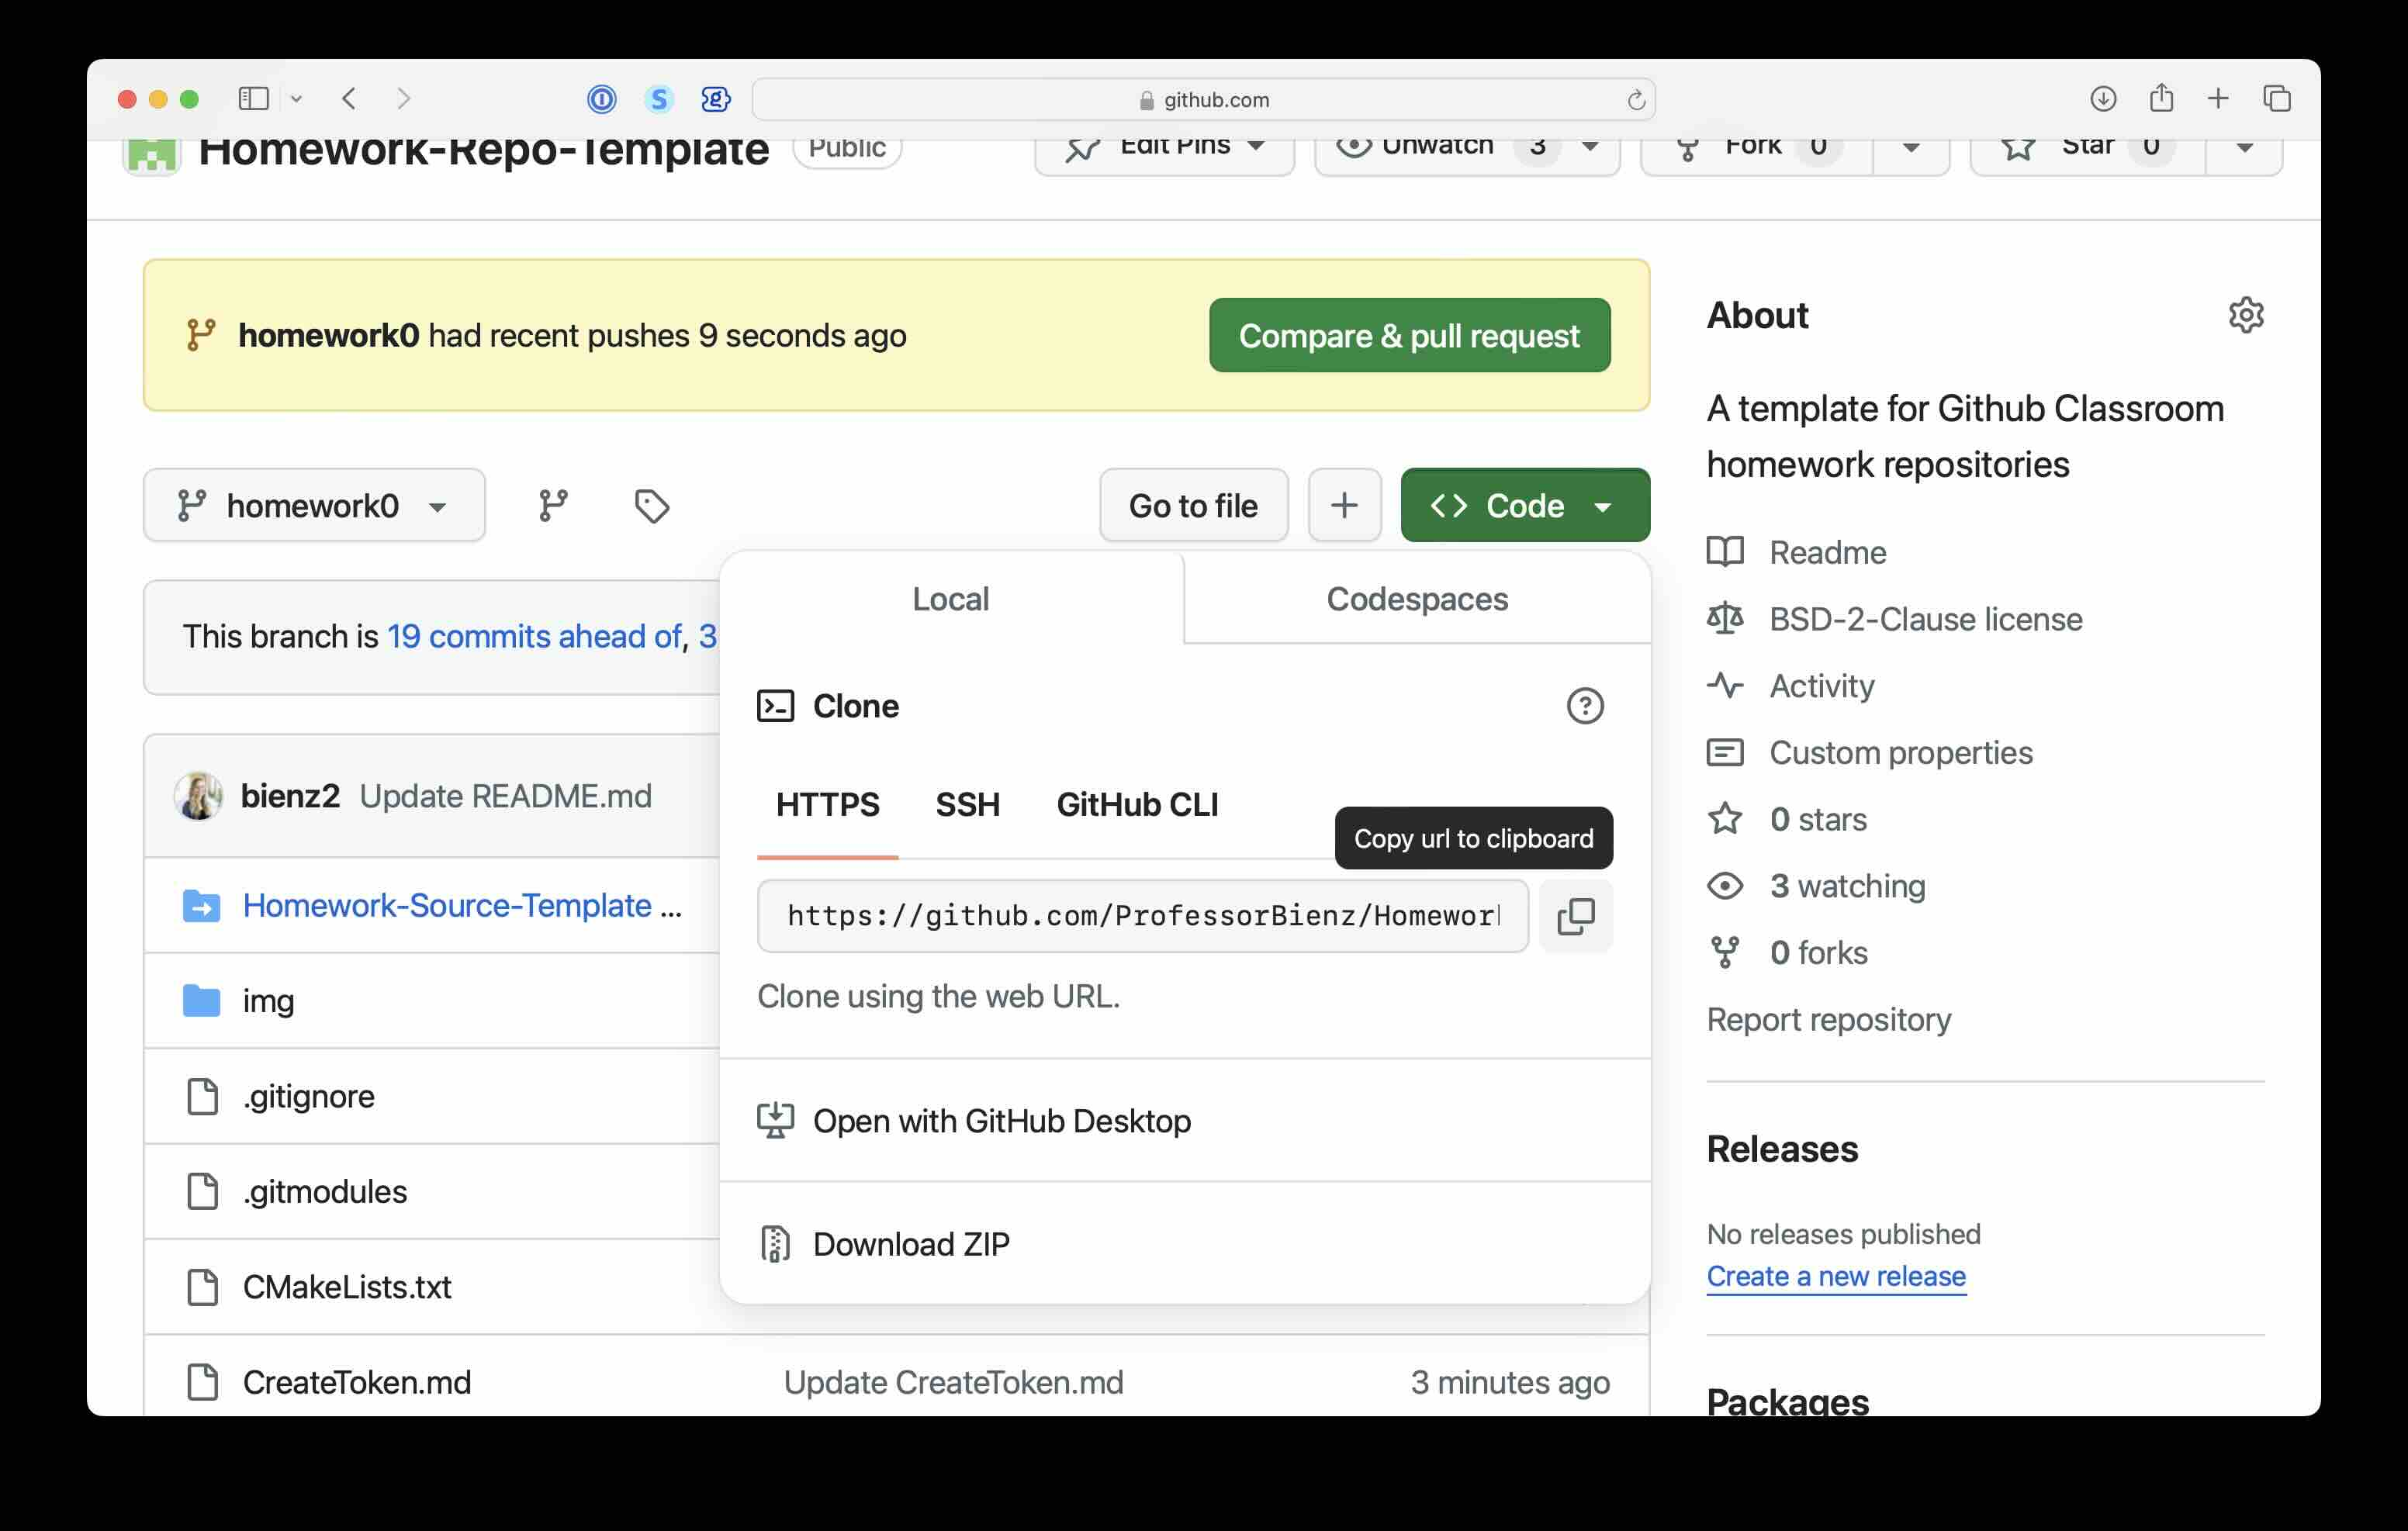
\includegraphics[width=0.75\textwidth]{figs/0_repo_addr.jpg}

    \item [(1.3:)] After you clone your repository, you should see similar output.  If you get an error, check your that you have correctly copied the HTTPS address from your repository.  If you are asked for a password, you need to use your GitHub authentication token, not your main GitHub password.\\  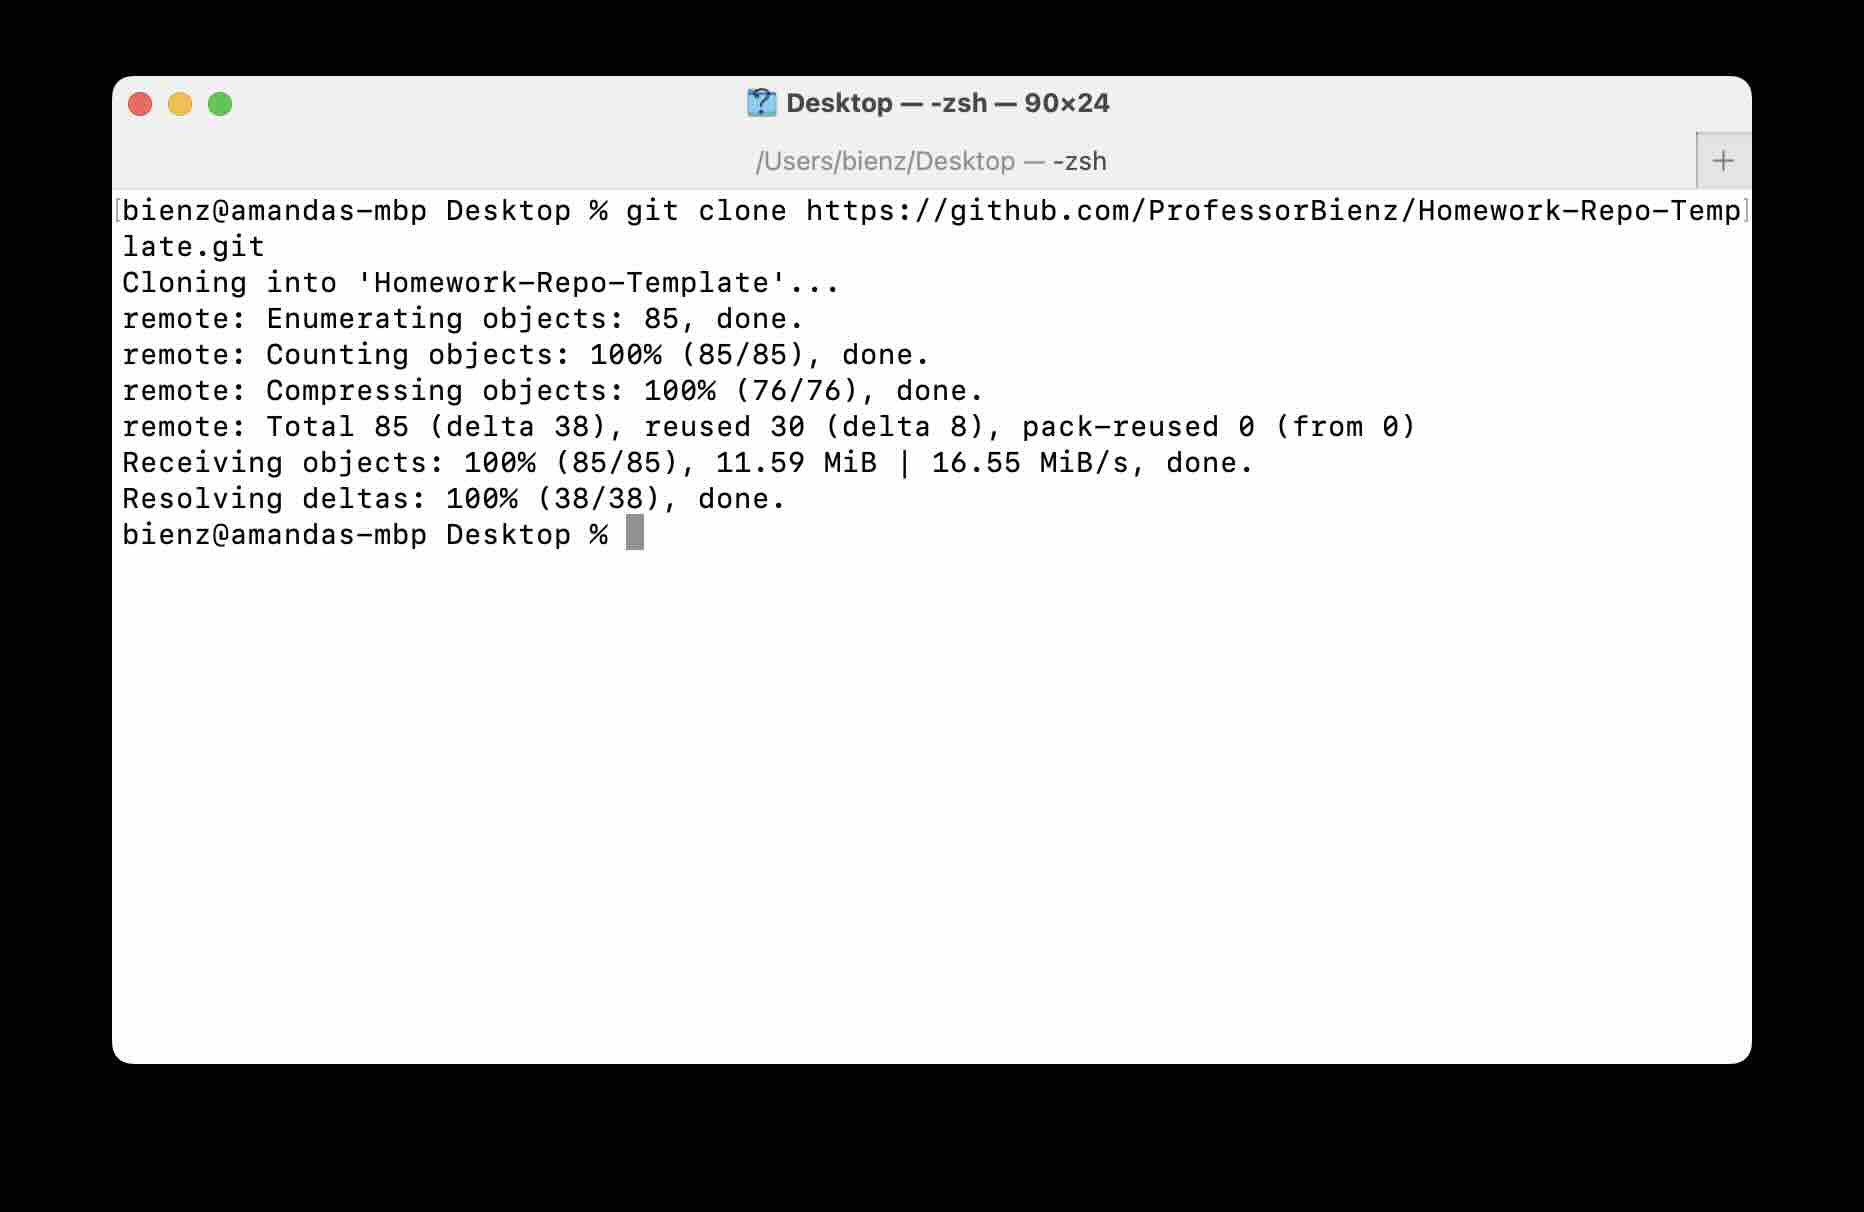
\includegraphics[width=0.75\textwidth]{figs/1_clone.jpg}

    \item [(1.5)] After you update your submodule, you may see similar output to the image below.  However, if your submodule was already up-to-date, you will see no output when you type this command.\\
    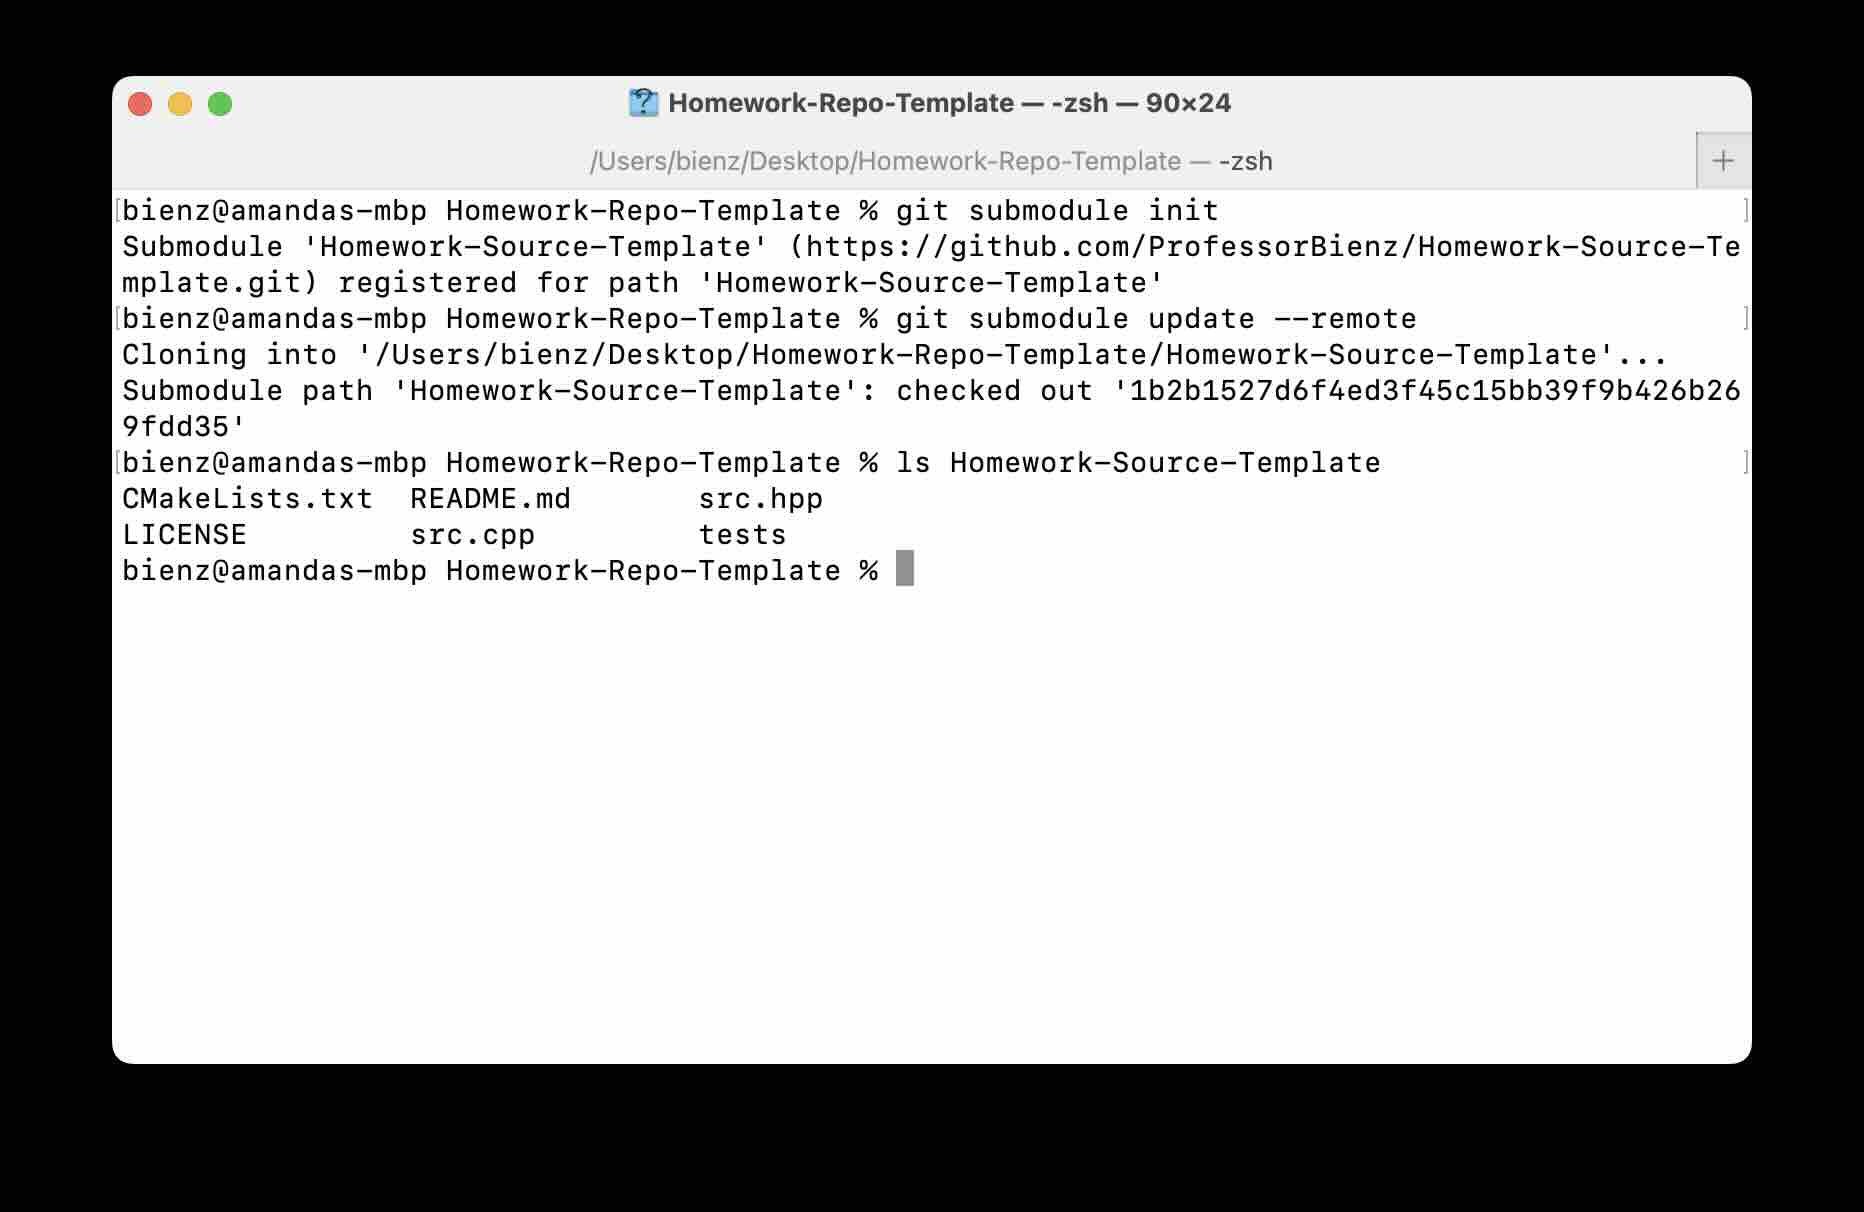
\includegraphics[width=0.75\textwidth]{figs/4_submodule.jpg}

    \item [(2.3)] The following image shows how to create a new build folder, move into that folder, and run the `cmake` configuration script from within that folder.  \textbf{Make sure you have two dots after cmake, pointing to the CMakeLists.txt file, which is in the parent directory of your current location (the build folder).}\\
    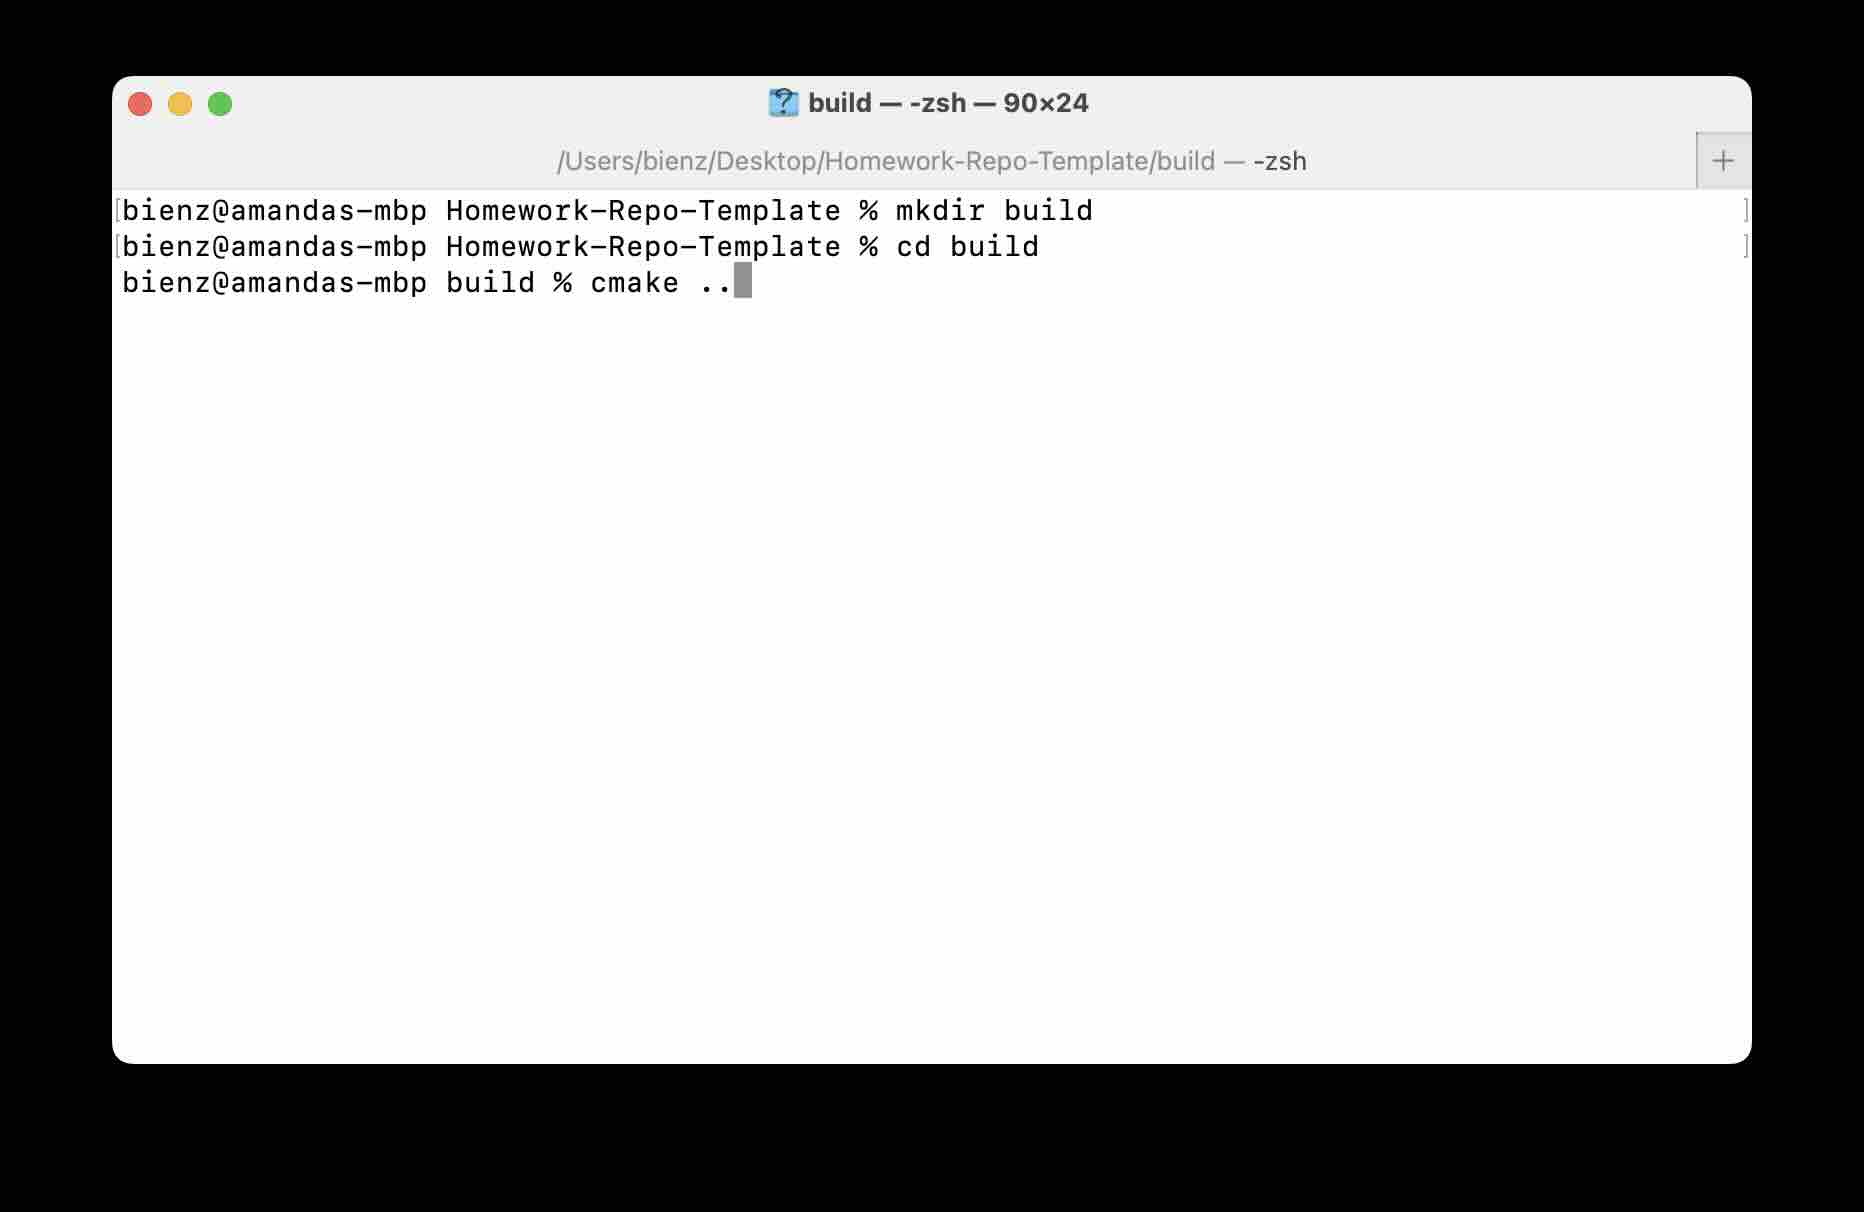
\includegraphics[width=0.75\textwidth]{figs/5_configure.jpg}\\
    CMake will configure your code, and you should see the line saying `Build files have been written to...`, pointing to a location on your computer.  You may see warnings and that is okay, but you should not see any CMake errors.\\
    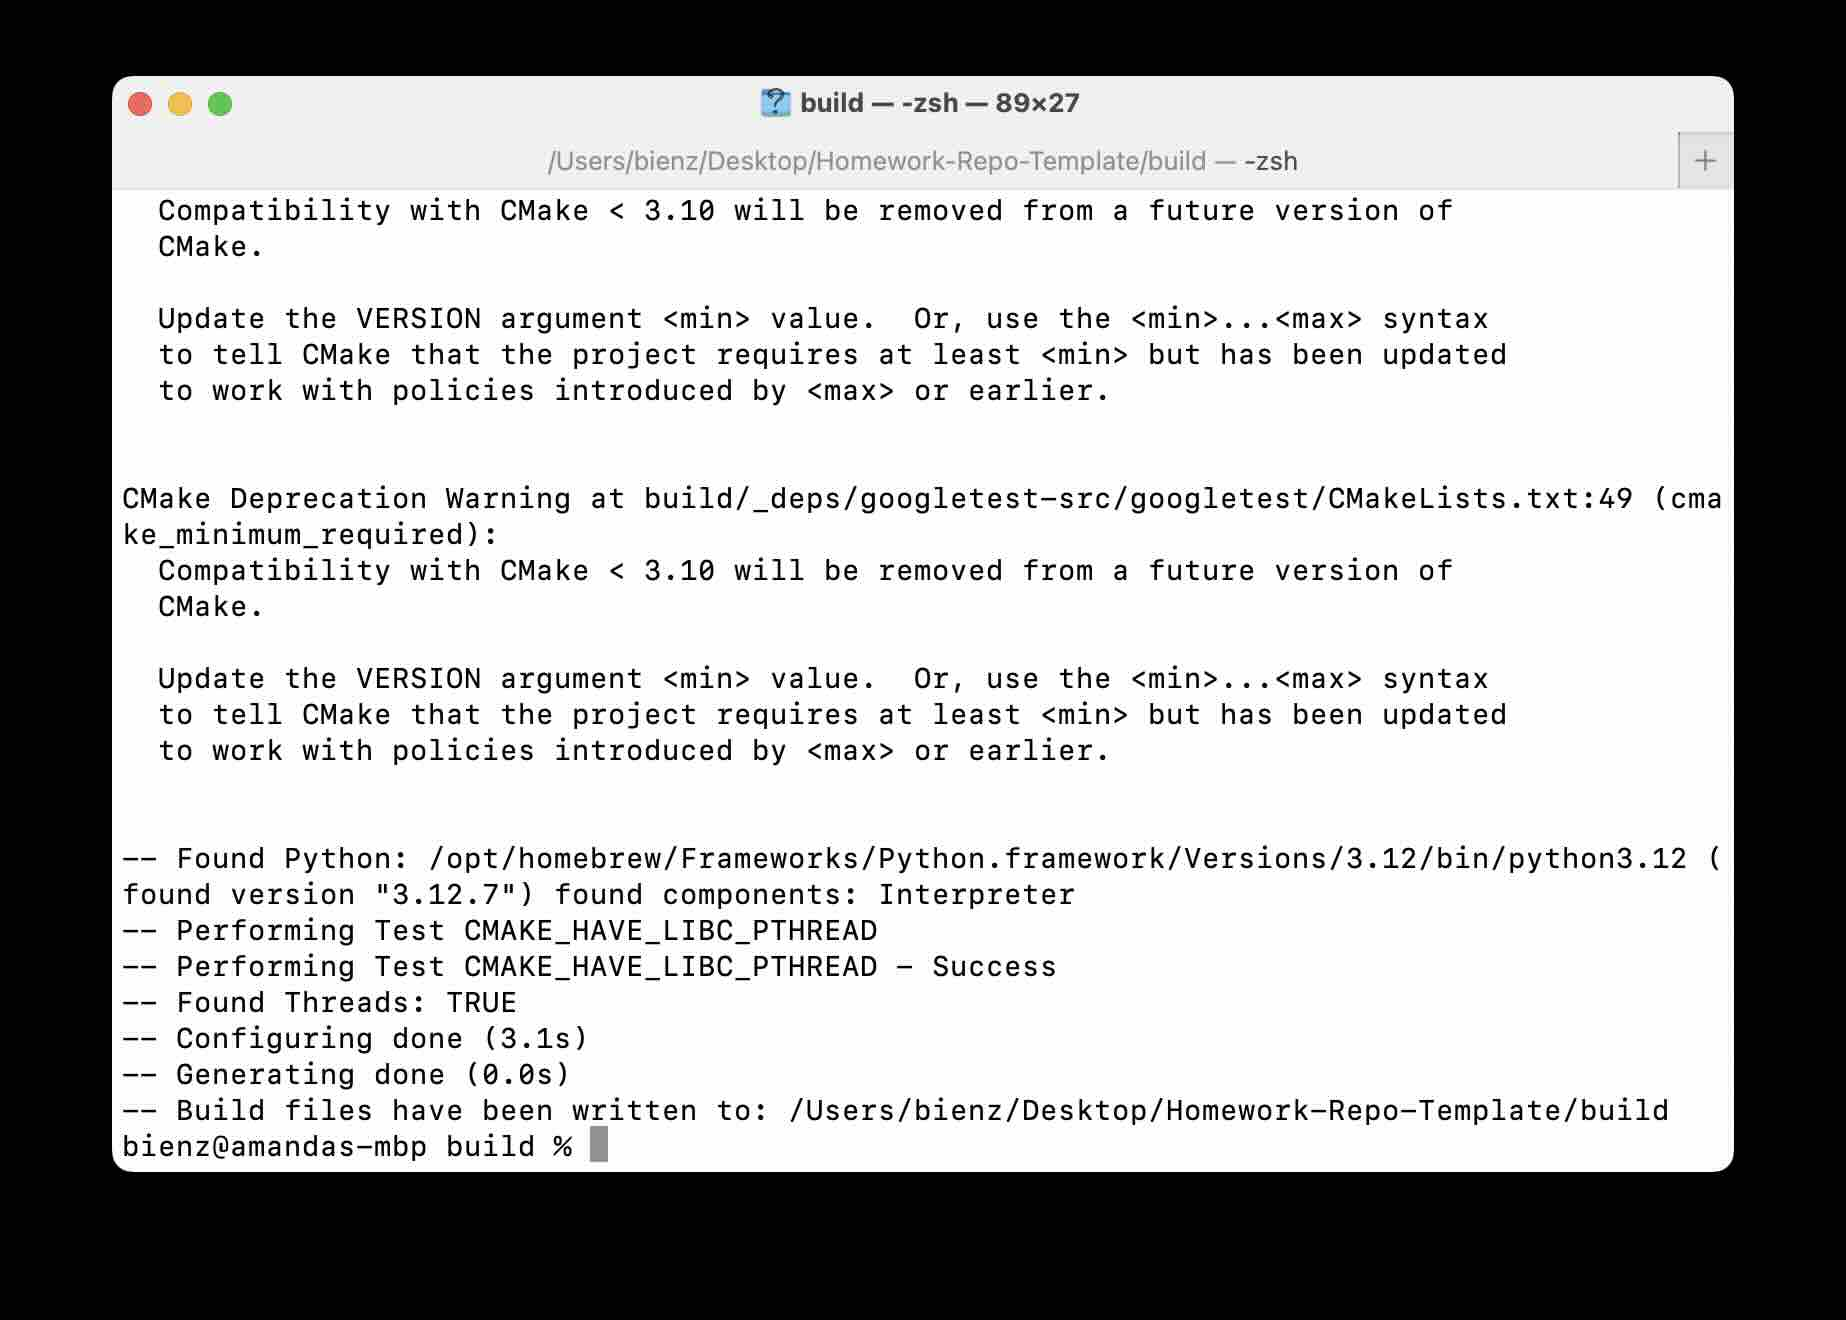
\includegraphics[width=0.75\textwidth]{figs/6_configure.jpg}

    \item [(2.4)] When you compile your code, you should see files being built and linked.  You should also initially see an error at the end.  After you create your new function (step 2.5), and add it to the CMakeLists.txt (step 2.7), this error should go away.\\
    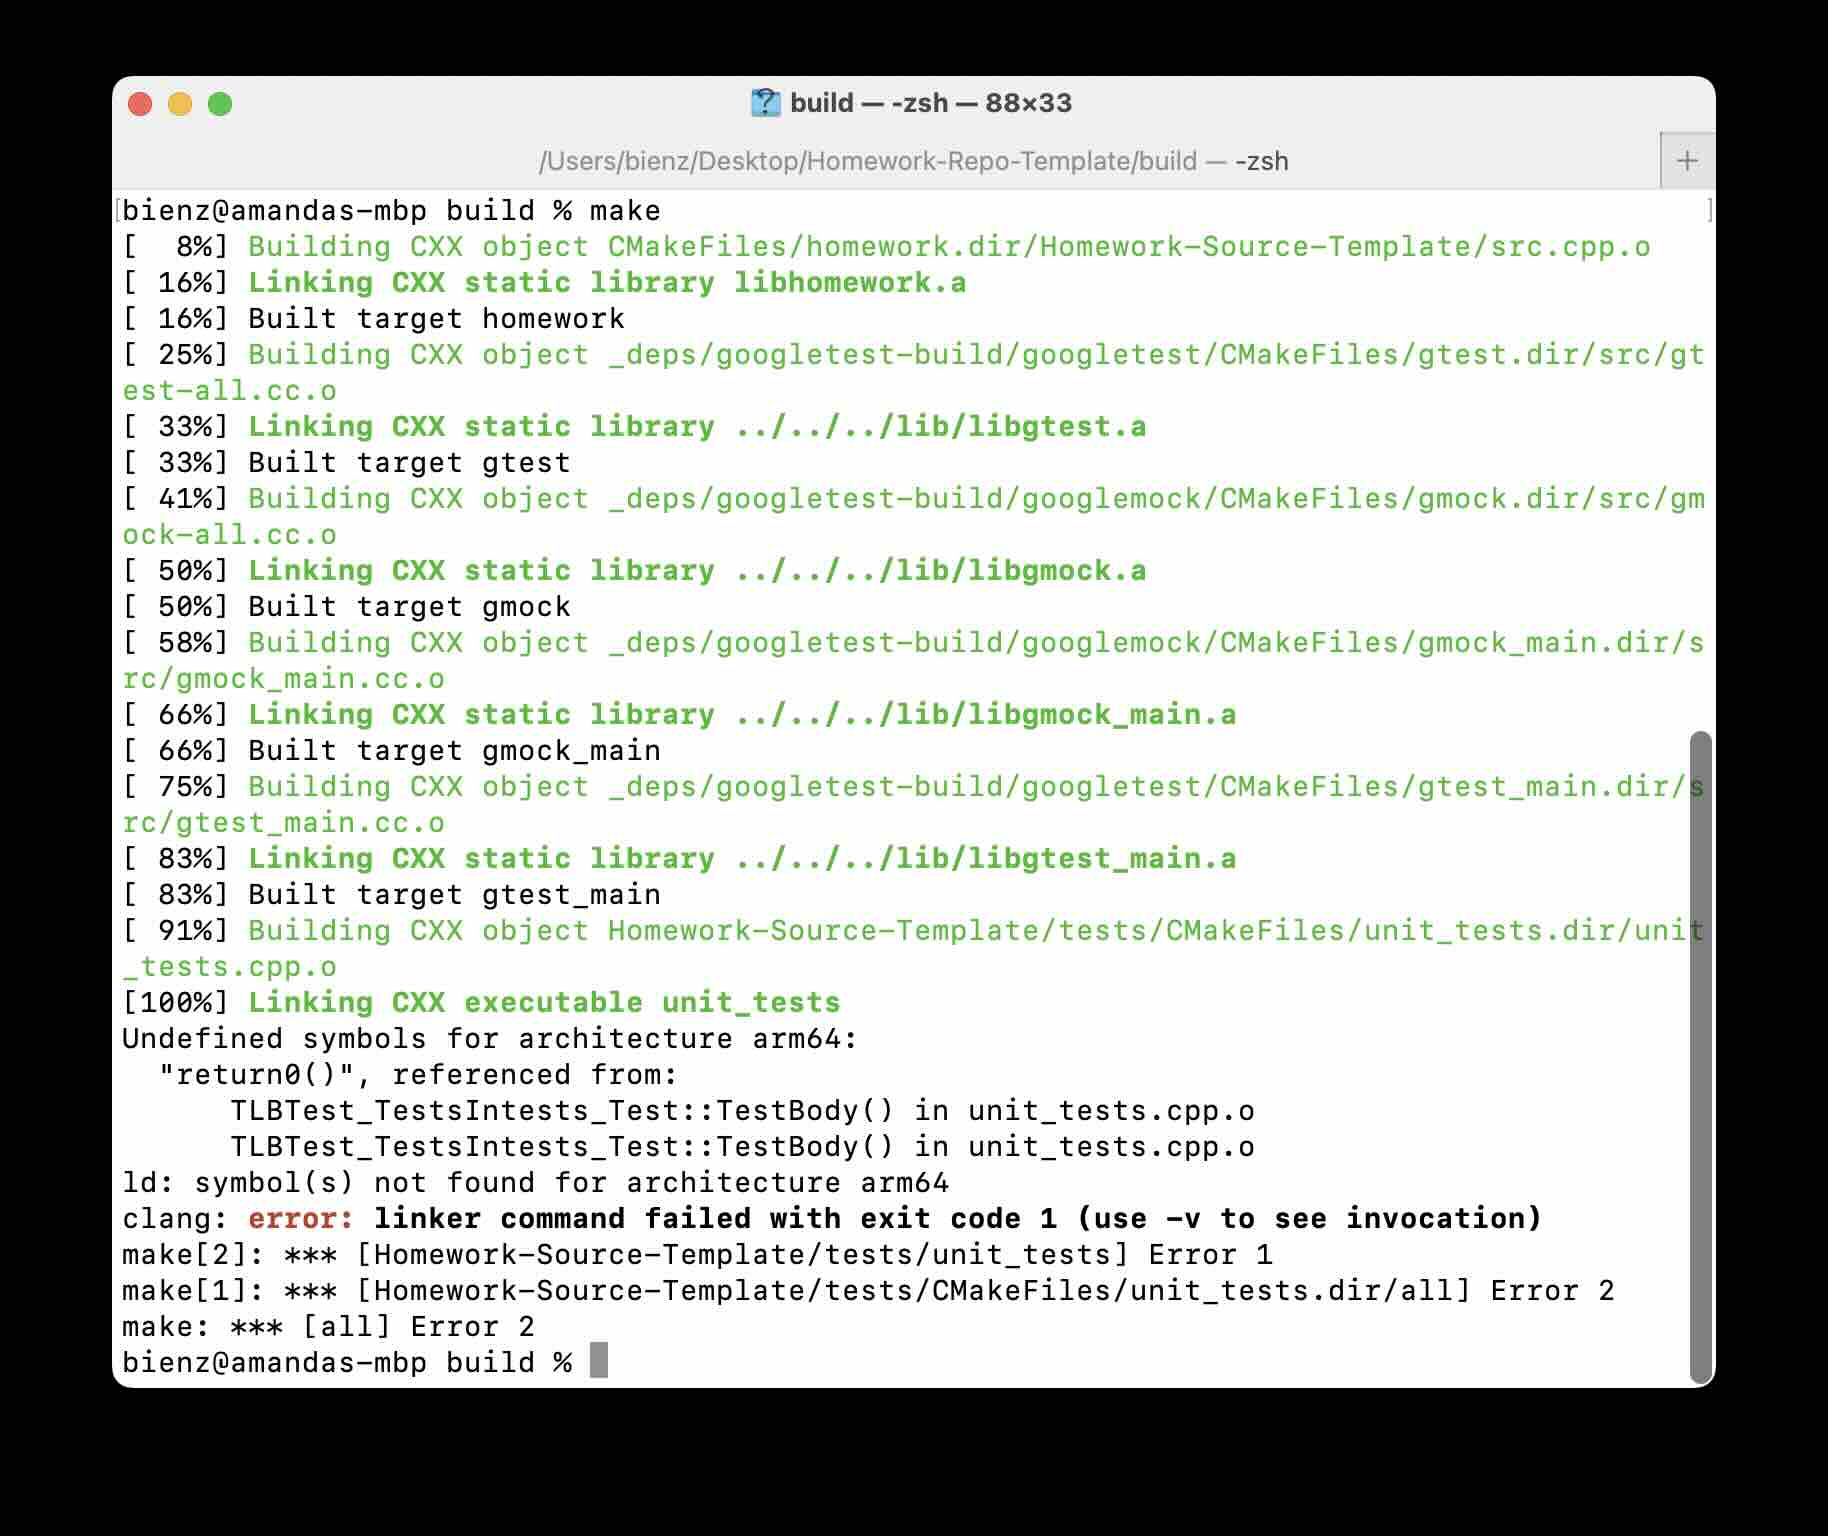
\includegraphics[width=0.75\textwidth]{figs/7_compile.jpg}

    \item [(2.5)] There are many options for creating a new file, including:
    \begin{itemize}
        \item `touch newfilename.cpp` will create a file that you can then edit with the editor of your choice.
        \item `vi newfilename.cpp` will create a new file and open it with VI, if installed.
        \item `emacs newfilename.cpp` will create a new file and open it with Emacs, if installed.
        \item Mac users: `mvim newfilename.cpp` will create a new file and open it with MacVim, if installed, allowing for both standard text editing and VI commands.
    \end{itemize}

    \item [(2.7)] This is what the CMakeLists.txt looks like.  If this is not what you see, you have opened the incorrect file.  Make sure you are opening the file CMakeLists.txt that is located within the main directory (not a file by the same name within the submodule).  \textbf{Add the .cpp file that you created either directly above or directly below the SRC\_SOURCES variable.}\\
    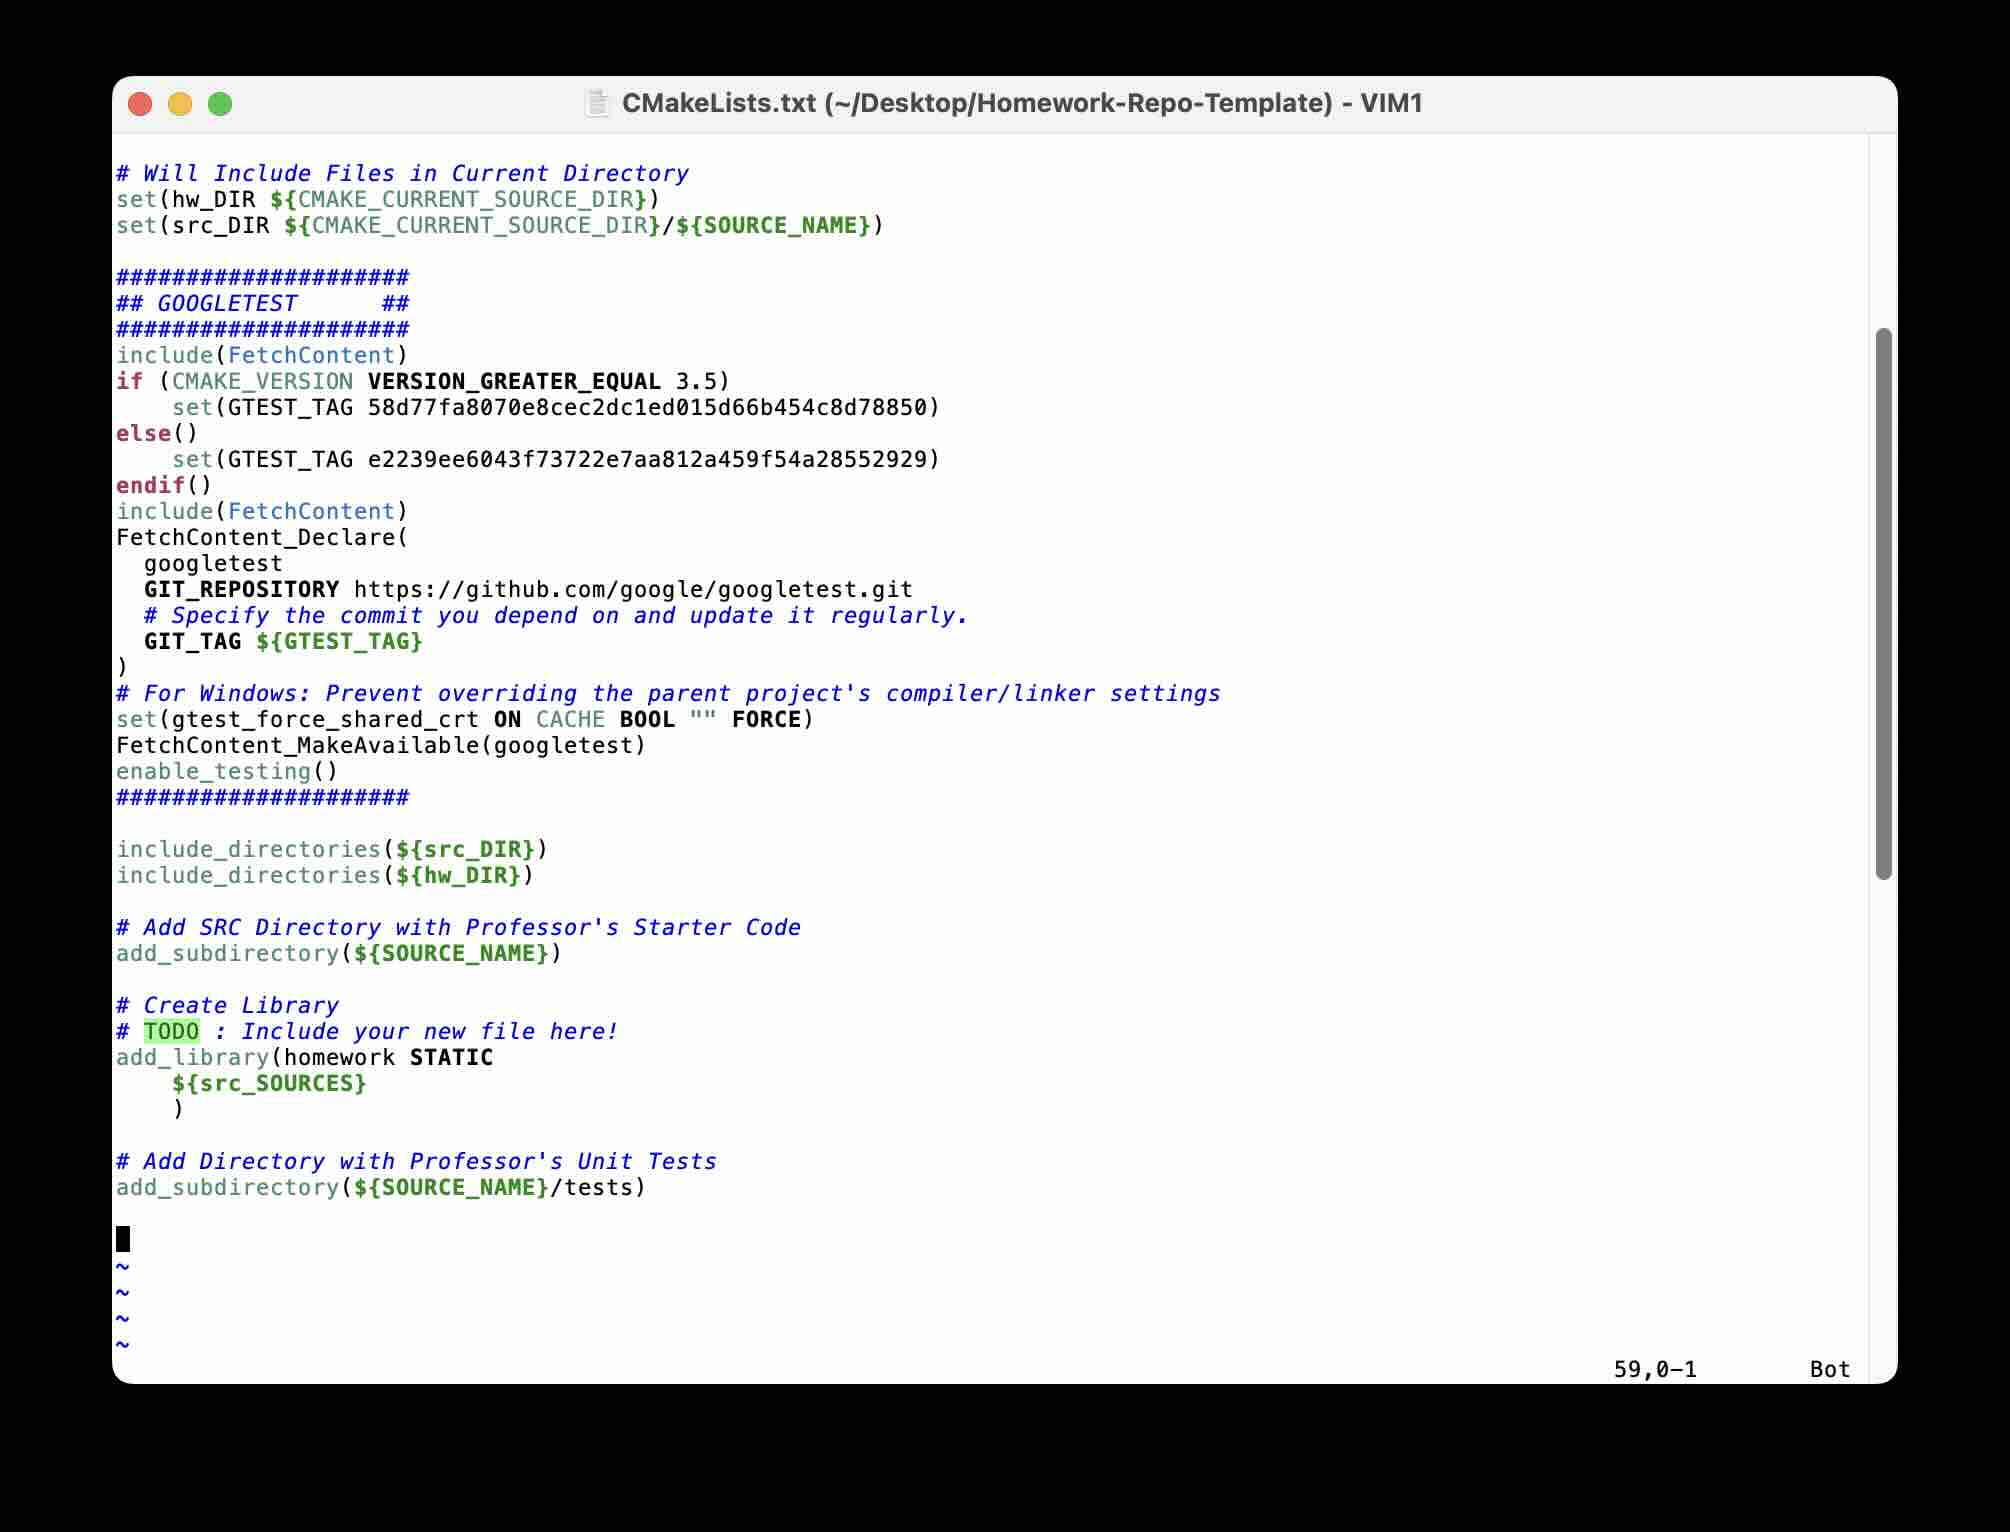
\includegraphics[width=0.75\textwidth]{figs/8_cmake.jpg}

    \item [(3.2)] Below is what the output of typing `make test` should look like.  If this is not what you see, check out common issues in the subsection below.\\
    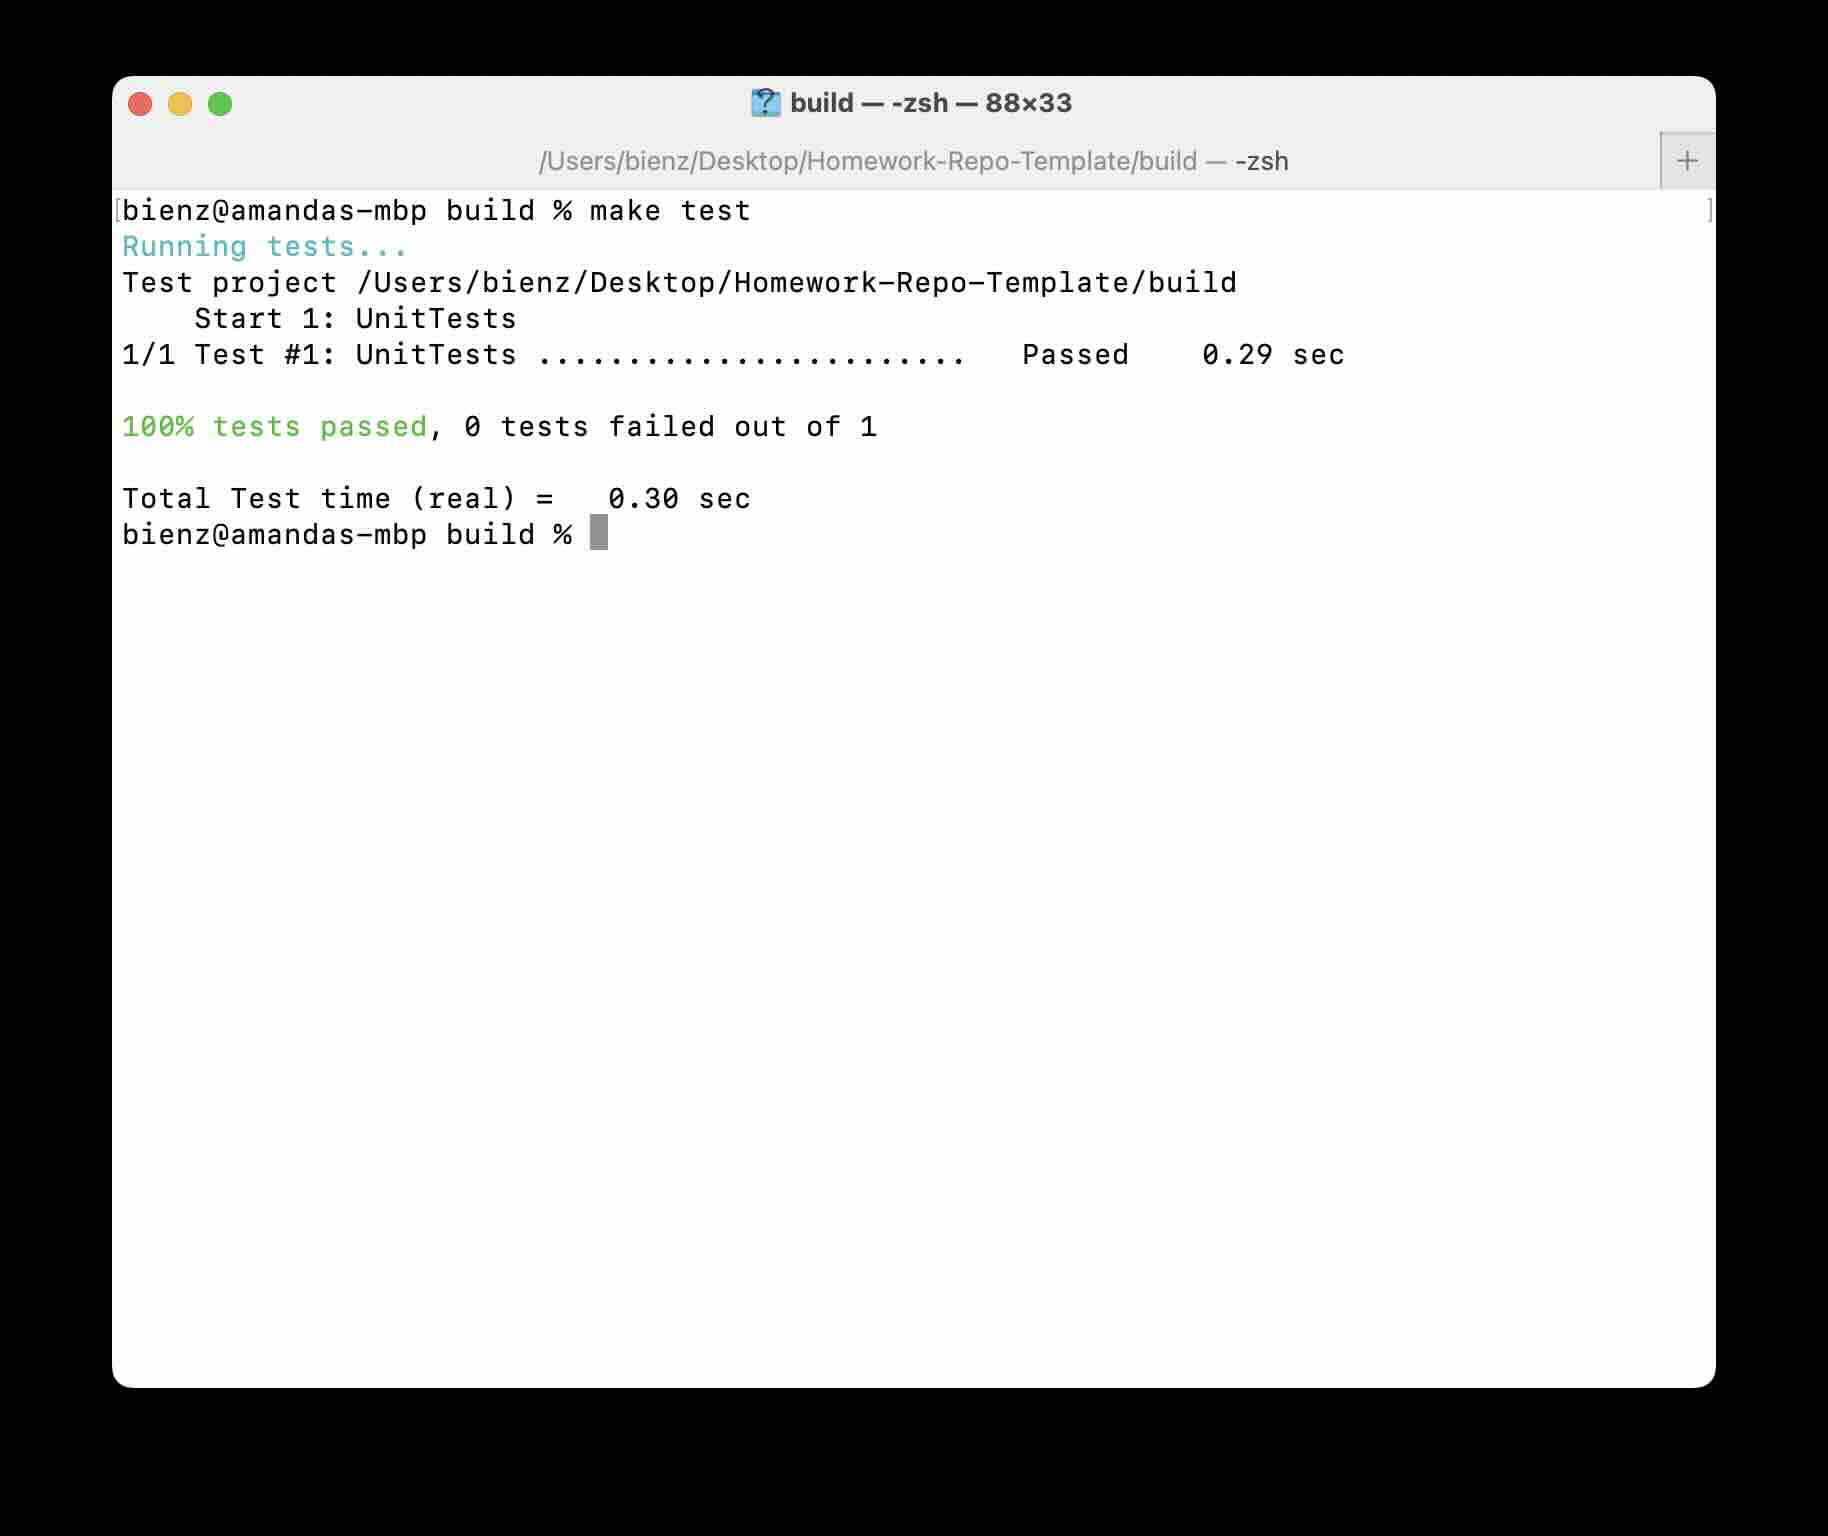
\includegraphics[width=0.75\textwidth]{figs/9_googletest.jpg}

    \item [(3.4)] This is what your `compile.sh` script should look like.\\
    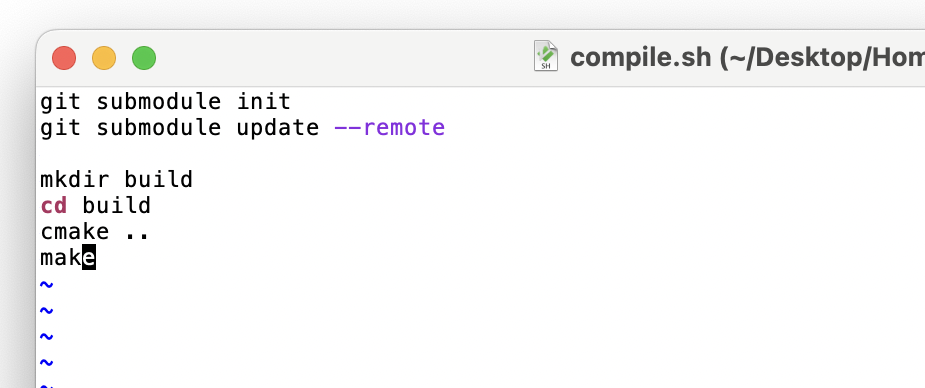
\includegraphics[width=0.75\textwidth]{figs/10config.png}

    \item [(4.8)] This is what you should see if you open up a passing GitHub actions test case (along with a green checkmark next to the Action).\\
    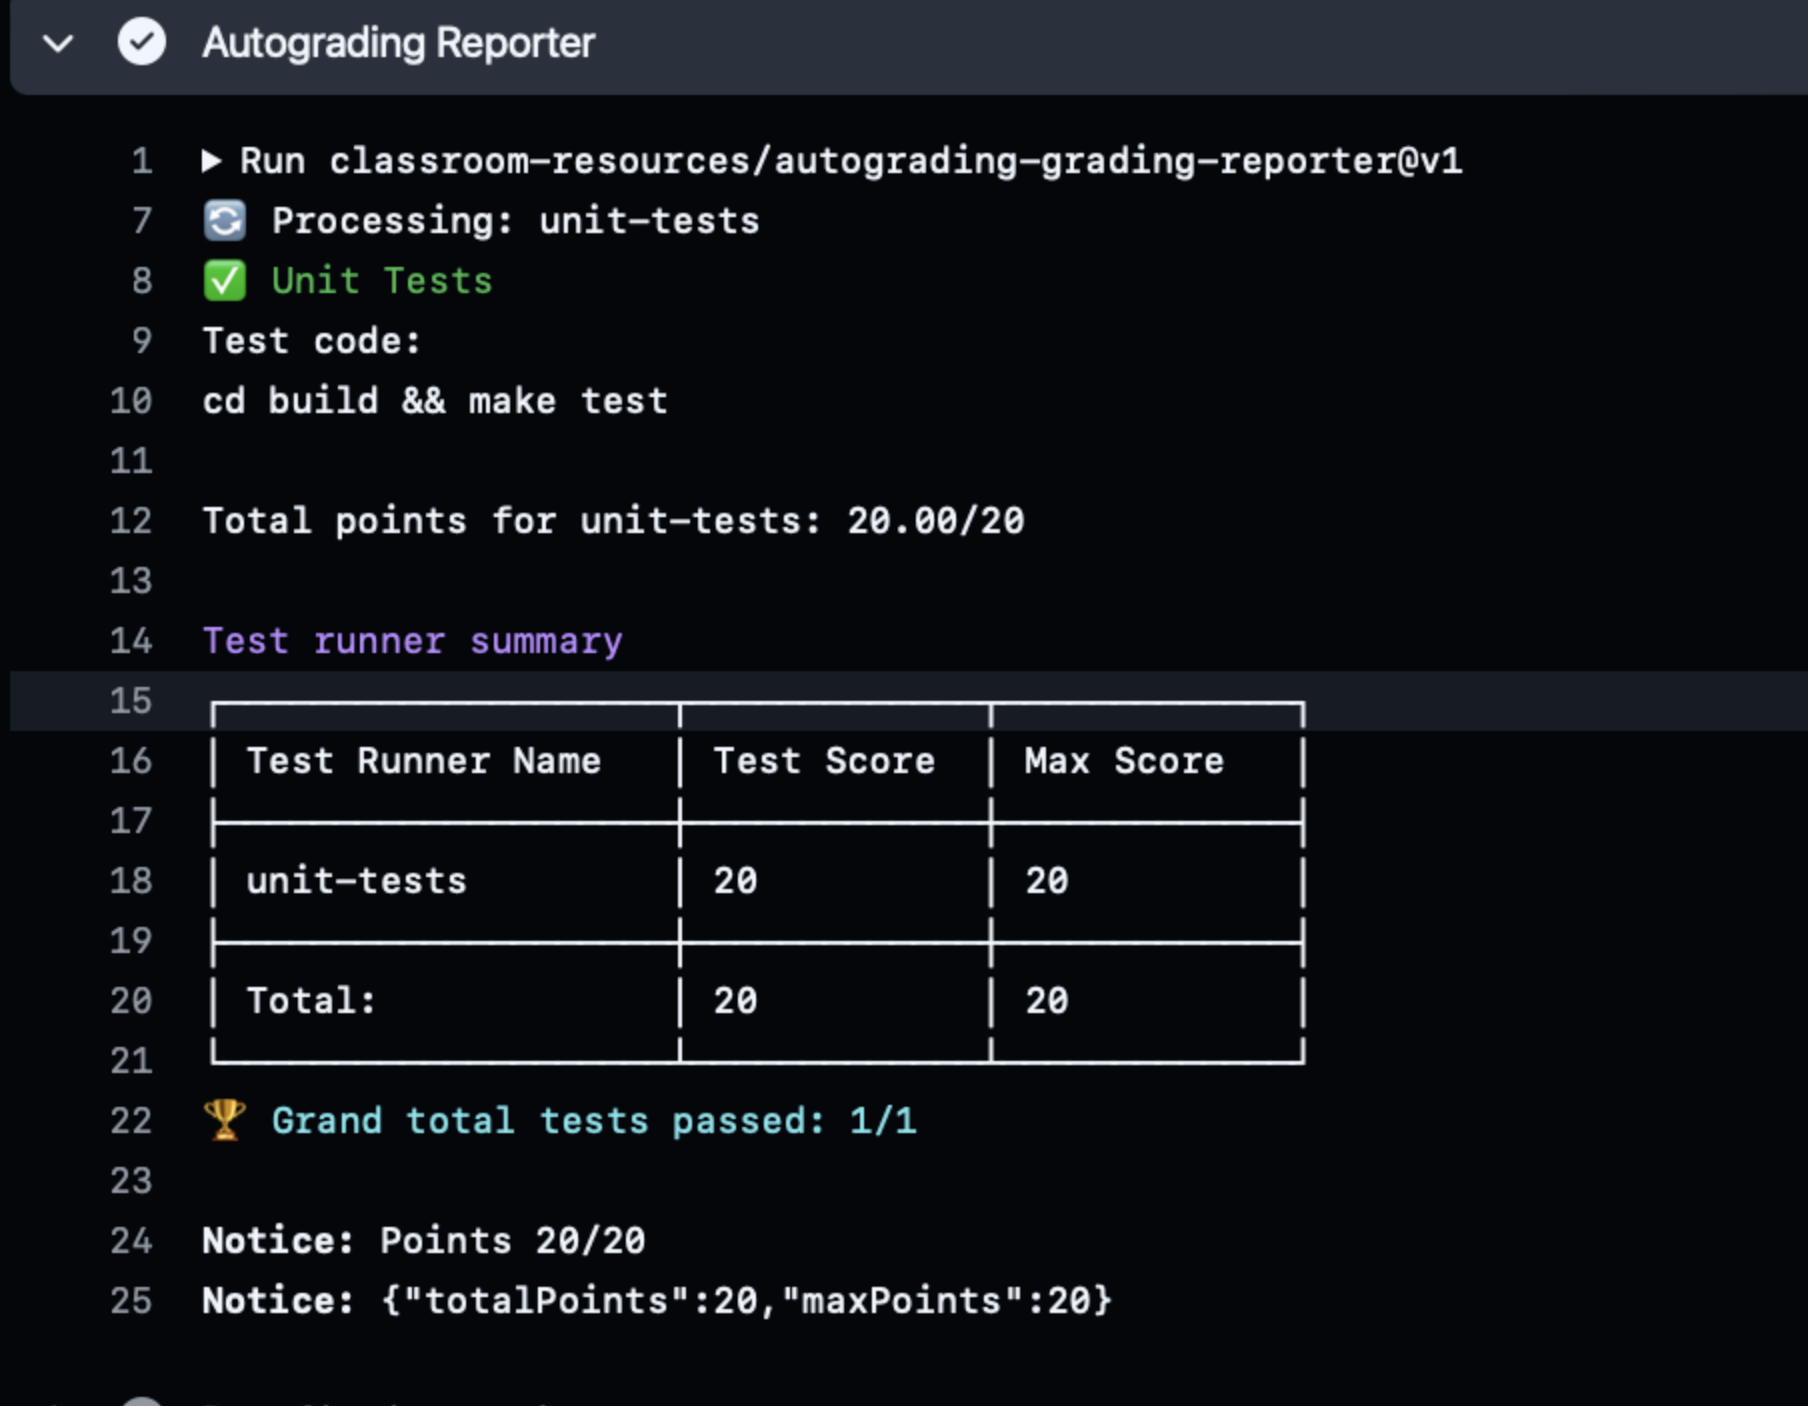
\includegraphics[width=0.75\textwidth]{figs/pass_autograder.png}\\
    If you click on the the dropdown arrow above the Autograding reporter, you should see the following.  If your test is not passing, you should click on the drop-down arrow to see why you are not passing, and check out common issues below for more information.\\
    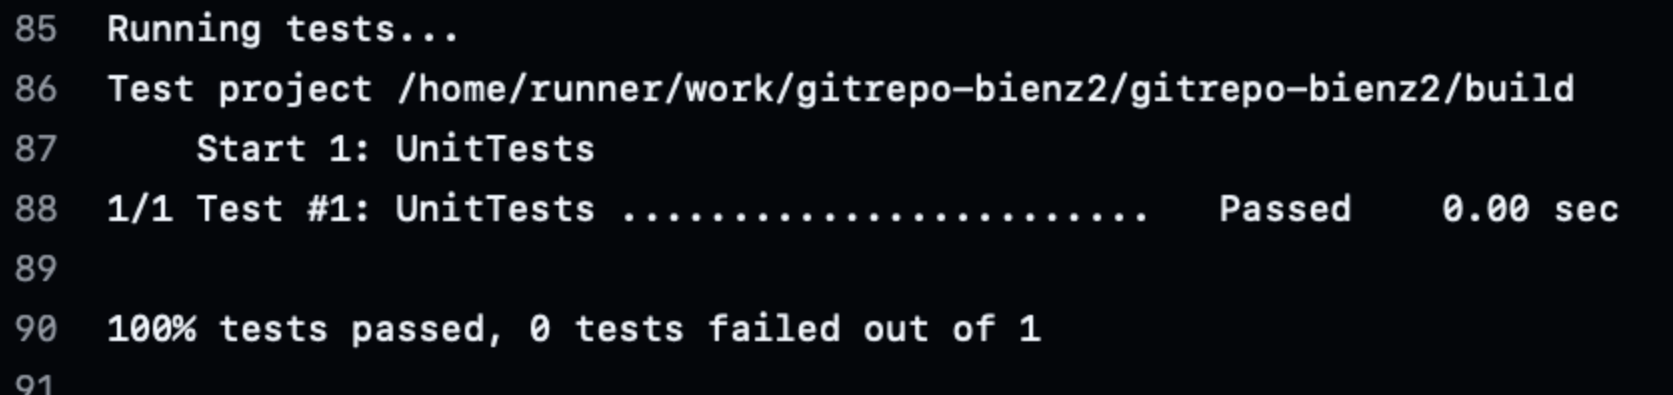
\includegraphics[width=0.75\textwidth]{figs/pass_test.png}
\end{enumerate}

\subsection*{Common Issues}
\begin{enumerate}
    \item \textbf{If you get an error while configuring or compiling the library:}
    \begin{itemize}
        \item If the error says CMake command not found, you need to install CMake.
        \item This may be due to an old cache.  Try removing everything from within the build directory, and then rerun your configure and compile commands.
        \item An error during the command `cmake ..` means there is an issue with your configuration.  Make sure you are running this command from the build directory and that the CMakeLists.txt file is in the parent directory.  If you still see an error, double check step 2.7.
        \item An error during the command `make` means there is an issue compiling your code.  Make sure you have a C/C++ compiler installed on your computer.  If you still see an error, double check step 2.6.
        \item If you are Windows, check the CMake on Windows bullet (\#6).
    \end{itemize}

    \item \textbf{If you get an error while running `make test`:}
    \begin{itemize}
        \item If your see tests similar to the image in the Hints above, check that your method `return0` returns the number 0.
        \item If you do not see `UnitTests` running, make sure you are running `make test` from within your build folder.
        \item If you still see an error, try running `make` and double check that your code compiles without error.
        \item If all else fails, try deleting and recreating your build directory.
    \end{itemize}

    \item \textbf{If you get an error in your GitHub Actions, click on the dropdown arrow for the individual tests (above your autograding report).  Some things you may find:}
    \begin{enumerate}
        \item `CMake Error` will point to the line within the `CMakeLists.txt` that an error is encountered.  If this includes `add\_subdirectory`, the issue is likely your submodule.  Go back and check that the code from Part 1, step 5 was added to your `compile.sh` file.\\
        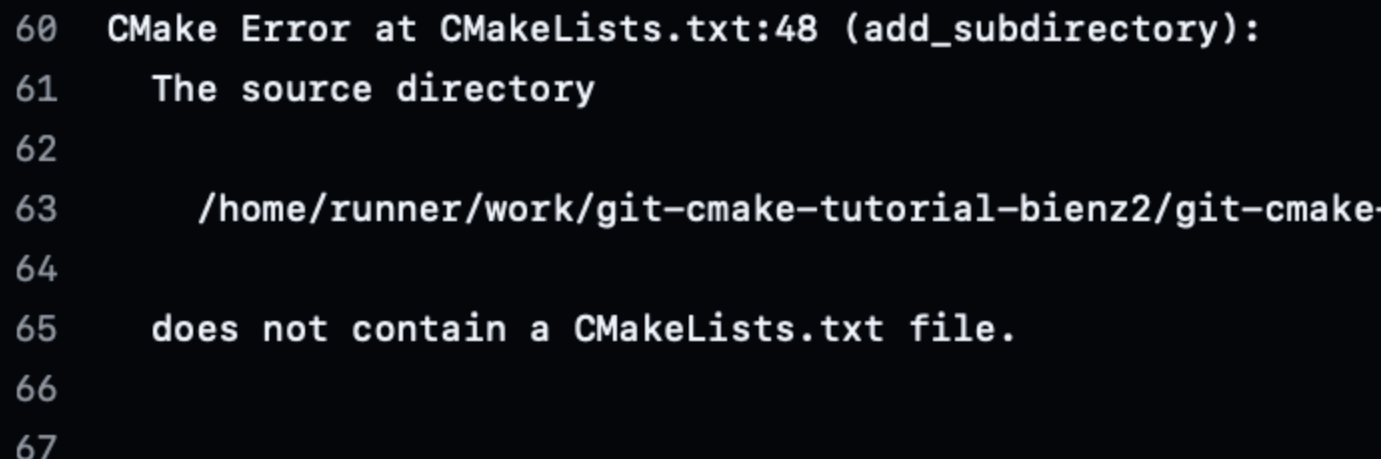
\includegraphics[width=0.75\textwidth]{figs/error_submodule.png}

        \item `Cannot find source file` means you are trying to compile code but cannot find the file.  Make sure you have added/committed/pushed the new file that you created.\\
        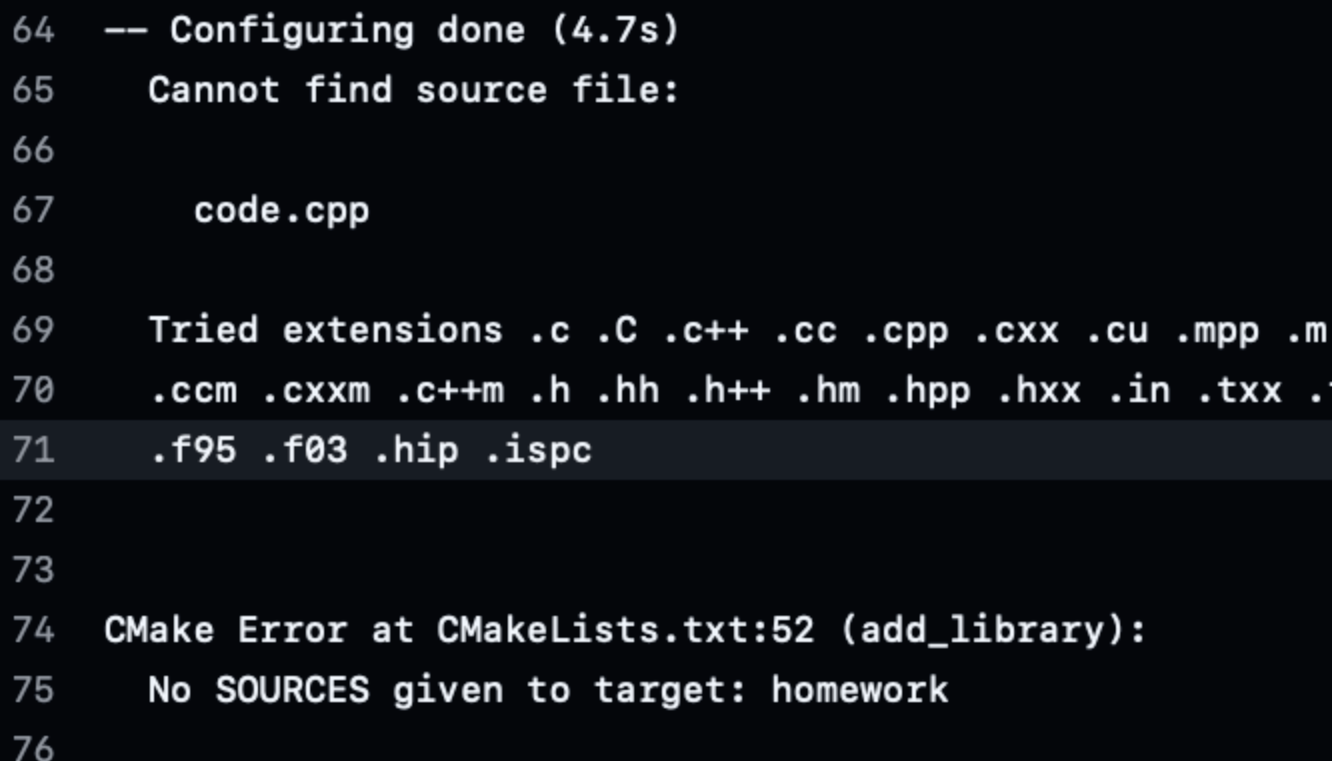
\includegraphics[width=0.75\textwidth]{figs/error_code.png}

        
        \item If your unit test fails, your return0 function does not return the number 0.\\
        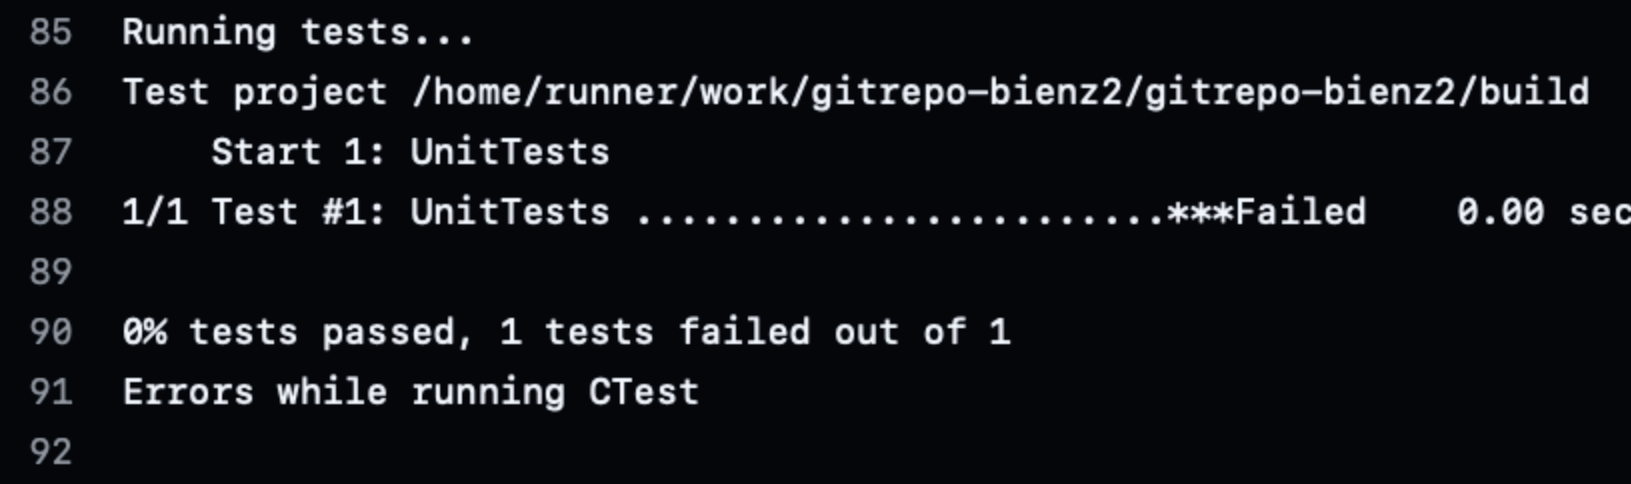
\includegraphics[width=0.75\textwidth]{figs/error_test.png}
    \end{enumerate}

    \item \textbf{Files Not Pushed.}  If you have a file on your computer and it is not showing up in your online repository, there are many possible reasons.  Type `git status` and check if you see any of the following:

    \begin{enumerate}
        \item The image below indicates you have changed the file `CMakeLists.txt`.  Add this updated file, commit, and push.\\
        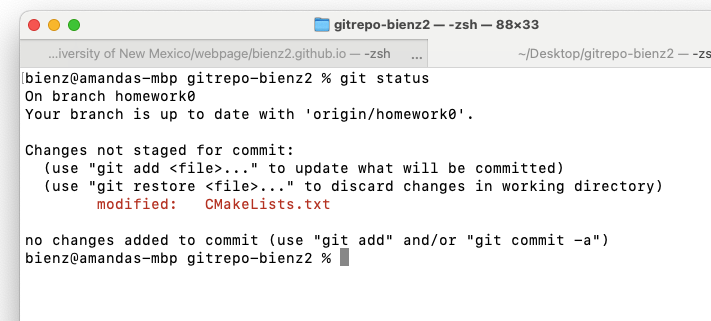
\includegraphics[width=0.75\textwidth]{figs/updates.png}

        \item The image below indicates you have created a new file `code.cpp`.  The command `git add -u` will not add this file, as it is untracked.  You need to type `git add code.cpp`.  Then, you will be able to commit and push the file.\\
        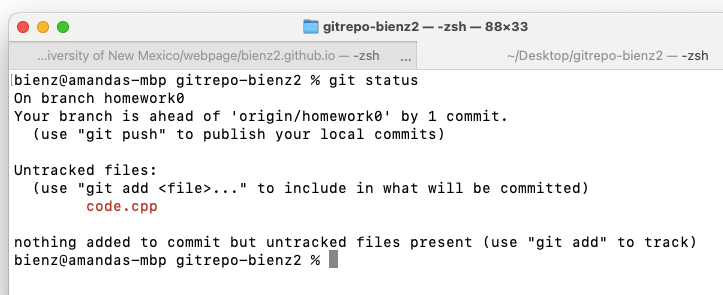
\includegraphics[width=0.75\textwidth]{figs/untracked.png}

        \item The image below indicates you have already added files, but have not committed or pushed.  Commit and push these files.\\
        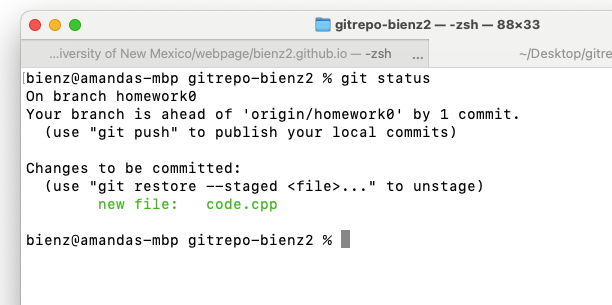
\includegraphics[width=0.75\textwidth]{figs/added.png}

        \item The image below indicates you have already committed files, but have not pushed.  Push these files.  Hint: there are no colors here.  The indication that you have committed is that `your branch is ahead of origin`, where `origin` is the online repository.\\
        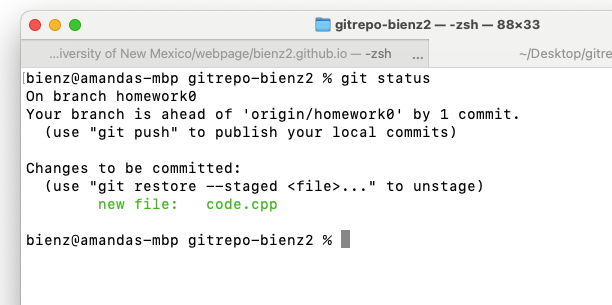
\includegraphics[width=0.75\textwidth]{figs/added.png}

        \item If all updated files have been committed and pushed, your repository should look like the following.\\
        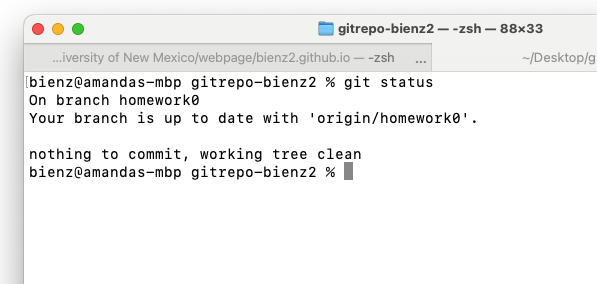
\includegraphics[width=0.75\textwidth]{figs/clean_dir.png}
    \end{enumerate}
    
    \item \textbf{Branch Issues:} If your status shows all files have been pushed, type `git branch`.  This should only show one branch.  

    \begin{enumerate}
        \item If instead you see HEAD detached, this means you are no longer appropriately connected to your GitHub repository. \\
        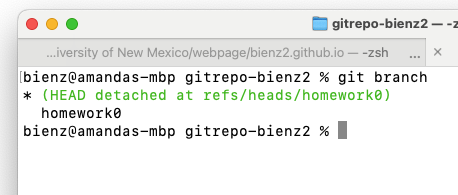
\includegraphics[width=0.75\textwidth]{figs/detached.png}    
    
        \item To fix this, you can create a new branch and merge it into the correct branch, as shown in the following image.\\
        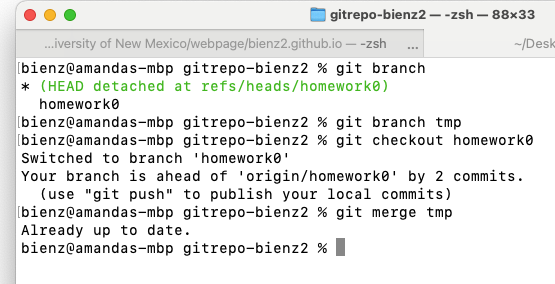
\includegraphics[width=0.75\textwidth]{figs/fix_detached.png}
    \end{enumerate}

    \item \textbf{CMake on Windows:} If you are using a Windows machine and get an error when configuring with `cmake ..`, try the following:
    \begin{enumerate}
        \item If you see an error `nmake' `-?' failed with: no such file or directory, CMake is unable to find the Make program on your computer.  Try adding the following between `cmake' and `..':\begin{verbatim}    
        -DCMAKE\_MAKE\_PROGRAM=mingw32-make -G "MinGW Makefiles"
        \end{verbatim}
        \item If you see an error `CMAKE\_CXX\_COMPILER not set', CMake is unable to determine which C compiler it should use.  Try adding the following between `cmake' and `..':\begin{verbatim}    
        -DCMAKE\_CXX\_COMPILER=g++
        \end{verbatim}
        Add `DCMAKE\_CXX\_COMPILER=g++' between `cmake' and `..'
        \item If you see an error `CMAKE\_C\_COMPILER not set', CMake is unable to determine which C compiler it should use.  Try adding the following between `cmake' and `..':\begin{verbatim}    
        -DCMAKE\_CXX\_COMPILER=gcc
        \end{verbatim}
    \end{enumerate}
    If you see all three errors above, your CMake configure line would be \begin{verbatim}
        cmake -DCMAKE_CXX_COMPILER=g++ -DCMAKE_CC_COMPILER=gcc 
        -DCMAKE_MAKE_PROGRAM=mingw32-make -G "MinGW Makefiles" ..
    \end{verbatim}

    \item \textbf{Make on Windows} If you run into issues on Windows where the flags from the previous step allowed you to configure (CMake passed) but you get an error that `make' command not found, try the following command instead 
    \begin{verbatim}
        mingw32-make
    \end{verbatim}
\end{enumerate}

\end{document}

